% Options for packages loaded elsewhere
\PassOptionsToPackage{unicode}{hyperref}
\PassOptionsToPackage{hyphens}{url}
\PassOptionsToPackage{dvipsnames,svgnames,x11names}{xcolor}
%
\documentclass[
]{article}
\usepackage{amsmath,amssymb}
\usepackage{iftex}
\ifPDFTeX
  \usepackage[T1]{fontenc}
  \usepackage[utf8]{inputenc}
  \usepackage{textcomp} % provide euro and other symbols
\else % if luatex or xetex
  \usepackage{unicode-math} % this also loads fontspec
  \defaultfontfeatures{Scale=MatchLowercase}
  \defaultfontfeatures[\rmfamily]{Ligatures=TeX,Scale=1}
\fi
\usepackage{lmodern}
\ifPDFTeX\else
  % xetex/luatex font selection
\fi
% Use upquote if available, for straight quotes in verbatim environments
\IfFileExists{upquote.sty}{\usepackage{upquote}}{}
\IfFileExists{microtype.sty}{% use microtype if available
  \usepackage[]{microtype}
  \UseMicrotypeSet[protrusion]{basicmath} % disable protrusion for tt fonts
}{}
\makeatletter
\@ifundefined{KOMAClassName}{% if non-KOMA class
  \IfFileExists{parskip.sty}{%
    \usepackage{parskip}
  }{% else
    \setlength{\parindent}{0pt}
    \setlength{\parskip}{6pt plus 2pt minus 1pt}}
}{% if KOMA class
  \KOMAoptions{parskip=half}}
\makeatother
\usepackage{xcolor}
\usepackage[margin=1in]{geometry}
\usepackage{color}
\usepackage{fancyvrb}
\newcommand{\VerbBar}{|}
\newcommand{\VERB}{\Verb[commandchars=\\\{\}]}
\DefineVerbatimEnvironment{Highlighting}{Verbatim}{commandchars=\\\{\}}
% Add ',fontsize=\small' for more characters per line
\usepackage{framed}
\definecolor{shadecolor}{RGB}{248,248,248}
\newenvironment{Shaded}{\begin{snugshade}}{\end{snugshade}}
\newcommand{\AlertTok}[1]{\textcolor[rgb]{0.94,0.16,0.16}{#1}}
\newcommand{\AnnotationTok}[1]{\textcolor[rgb]{0.56,0.35,0.01}{\textbf{\textit{#1}}}}
\newcommand{\AttributeTok}[1]{\textcolor[rgb]{0.13,0.29,0.53}{#1}}
\newcommand{\BaseNTok}[1]{\textcolor[rgb]{0.00,0.00,0.81}{#1}}
\newcommand{\BuiltInTok}[1]{#1}
\newcommand{\CharTok}[1]{\textcolor[rgb]{0.31,0.60,0.02}{#1}}
\newcommand{\CommentTok}[1]{\textcolor[rgb]{0.56,0.35,0.01}{\textit{#1}}}
\newcommand{\CommentVarTok}[1]{\textcolor[rgb]{0.56,0.35,0.01}{\textbf{\textit{#1}}}}
\newcommand{\ConstantTok}[1]{\textcolor[rgb]{0.56,0.35,0.01}{#1}}
\newcommand{\ControlFlowTok}[1]{\textcolor[rgb]{0.13,0.29,0.53}{\textbf{#1}}}
\newcommand{\DataTypeTok}[1]{\textcolor[rgb]{0.13,0.29,0.53}{#1}}
\newcommand{\DecValTok}[1]{\textcolor[rgb]{0.00,0.00,0.81}{#1}}
\newcommand{\DocumentationTok}[1]{\textcolor[rgb]{0.56,0.35,0.01}{\textbf{\textit{#1}}}}
\newcommand{\ErrorTok}[1]{\textcolor[rgb]{0.64,0.00,0.00}{\textbf{#1}}}
\newcommand{\ExtensionTok}[1]{#1}
\newcommand{\FloatTok}[1]{\textcolor[rgb]{0.00,0.00,0.81}{#1}}
\newcommand{\FunctionTok}[1]{\textcolor[rgb]{0.13,0.29,0.53}{\textbf{#1}}}
\newcommand{\ImportTok}[1]{#1}
\newcommand{\InformationTok}[1]{\textcolor[rgb]{0.56,0.35,0.01}{\textbf{\textit{#1}}}}
\newcommand{\KeywordTok}[1]{\textcolor[rgb]{0.13,0.29,0.53}{\textbf{#1}}}
\newcommand{\NormalTok}[1]{#1}
\newcommand{\OperatorTok}[1]{\textcolor[rgb]{0.81,0.36,0.00}{\textbf{#1}}}
\newcommand{\OtherTok}[1]{\textcolor[rgb]{0.56,0.35,0.01}{#1}}
\newcommand{\PreprocessorTok}[1]{\textcolor[rgb]{0.56,0.35,0.01}{\textit{#1}}}
\newcommand{\RegionMarkerTok}[1]{#1}
\newcommand{\SpecialCharTok}[1]{\textcolor[rgb]{0.81,0.36,0.00}{\textbf{#1}}}
\newcommand{\SpecialStringTok}[1]{\textcolor[rgb]{0.31,0.60,0.02}{#1}}
\newcommand{\StringTok}[1]{\textcolor[rgb]{0.31,0.60,0.02}{#1}}
\newcommand{\VariableTok}[1]{\textcolor[rgb]{0.00,0.00,0.00}{#1}}
\newcommand{\VerbatimStringTok}[1]{\textcolor[rgb]{0.31,0.60,0.02}{#1}}
\newcommand{\WarningTok}[1]{\textcolor[rgb]{0.56,0.35,0.01}{\textbf{\textit{#1}}}}
\usepackage{graphicx}
\makeatletter
\def\maxwidth{\ifdim\Gin@nat@width>\linewidth\linewidth\else\Gin@nat@width\fi}
\def\maxheight{\ifdim\Gin@nat@height>\textheight\textheight\else\Gin@nat@height\fi}
\makeatother
% Scale images if necessary, so that they will not overflow the page
% margins by default, and it is still possible to overwrite the defaults
% using explicit options in \includegraphics[width, height, ...]{}
\setkeys{Gin}{width=\maxwidth,height=\maxheight,keepaspectratio}
% Set default figure placement to htbp
\makeatletter
\def\fps@figure{htbp}
\makeatother
\setlength{\emergencystretch}{3em} % prevent overfull lines
\providecommand{\tightlist}{%
  \setlength{\itemsep}{0pt}\setlength{\parskip}{0pt}}
\setcounter{secnumdepth}{5}
\usepackage[french]{babel}
\ifLuaTeX
  \usepackage{selnolig}  % disable illegal ligatures
\fi
\usepackage{bookmark}
\IfFileExists{xurl.sty}{\usepackage{xurl}}{} % add URL line breaks if available
\urlstyle{same}
\hypersetup{
  pdfauthor={Taqwa Ben Romdhane, Manal Derghal, Khalil Ounis},
  colorlinks=true,
  linkcolor={Maroon},
  filecolor={Maroon},
  citecolor={Blue},
  urlcolor={blue},
  pdfcreator={LaTeX via pandoc}}

\title{Analyse des algorithmes de Maximum Subarray 2D\\
\strut ~M2 Data Science Algorithmique}
\author{Taqwa Ben Romdhane, Manal Derghal, Khalil Ounis}
\date{Mercredi 9 avril 2025}

\begin{document}
\maketitle

{
\hypersetup{linkcolor=}
\setcounter{tocdepth}{2}
\tableofcontents
}
\noindent\hrulefill

\section{Description du problème et
objectif}\label{description-du-probluxe8me-et-objectif}

\subsection{Présentation du
problème}\label{pruxe9sentation-du-probluxe8me}

Dans ce document, nous étudions le problème du sous-tableau de somme
maximale du point de vue de la complexité algorithmique. Ce problème est
intéressant car il existe de nombreux algorithmes pour le résoudre, dont
la complexité varie considérablement.

Dans ce rapport, nous abordons uniquement deux algorithmes :

un algorithme naïf utilisant le paradigme de Brute Force,

et un algorithme optimal basé sur la méthode de Kadane.

Nous étendons ensuite le problème à deux dimensions afin de déterminer
la sous-matrice contiguë de somme maximale dans une matrice. Bien que ce
cas soit plus complexe, la méthode de Kadane peut également être adaptée
au cas 2D.

Comme pour le cas 1D, nous proposerons deux solutions pour résoudre le
problème de la sous-matrice de somme maximale.

\subsection{Objectifs :}\label{objectifs}

Dans le cadre de ce projet, nous devons répondre aux objectifs suivants:

\begin{itemize}
\item
  Evaluer la performance en temps d'exécution des solutions naive et
  optimale
\item
  Implémenter ces algorithmes en R et en C++ et évaluer le gain de temps
\item
  Valider la complexité théorique attenue par une régression linéaire
\end{itemize}

\section{Maximum Sum Submatrix}\label{maximum-sum-submatrix}

Étant donné un tableau 2D, la tâche consiste à trouver la sous-matrice
de somme maximale qu'il contient.

Imaginez que vous avez cette matrice 4x5 :

Le rectangle en vert présente la sous-matrice avec la somme maximale
égale à 29.

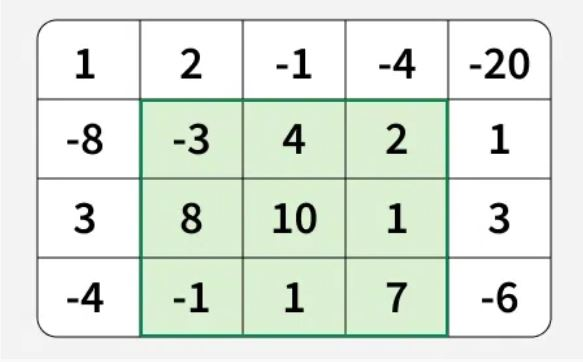
\includegraphics[width=1.85417in,height=\textheight]{images/G2-01.JPG}

\subsection{Approche naïve}\label{approche-nauxefve}

Nous explorons tous les rectangles possibles dans le tableau 2D donné,
en utilisant quatre variables : deux pour définir les limites gauche et
droite (\texttt{left} \& \texttt{right}), et deux autres pour définir
les limites supérieure et inférieure (\texttt{up} \& \texttt{down}).
Nous calculons leurs sommes et gardons une trace de la somme maximale
trouvée.

\textbf{Complexité algorithmique} :\\
\(O\left((nm)^3\right)\)\\
Nous parcourons toutes les limites du rectangle en \(O((nm)^2)\), et
pour chaque rectangle, nous calculons sa somme en \(O(nm)\). Par
conséquent, la complexité temporelle globale est \(O((nm)^3)\), où \(n\)
est le nombre de lignes et \(m\) le nombre de colonnes de la matrice.

Pour une matrice 3×3, il y a 36 sous-matrices. Si l'on étend cela à une
matrice 100×100, on obtient des millions de possibilités. Il est donc
clair que la méthode naïve de force brute ne fonctionne tout simplement
pas en pratique.

\subsection{Approche améliorée (Méthode de
Kadane)}\label{approche-amuxe9lioruxe9e-muxe9thode-de-kadane}

La nouvelle approche est basée sur l'algorithme de \textbf{Kadane}, qui
est utilisé comme solution optimale dans le cas 1D.\\
Nous allons expliquer comment appliquer cette méthode à un tableau 2D.\\
L'idée est de \textbf{compresser la matrice 2D en une série de tableaux
1D} et de résoudre chacun d'eux à l'aide de l'algorithme de Kadane.

\textbf{Complexité algorithmique} :\\
La complexité temporelle de cette approche est de \(O(n \cdot m^2)\), où
\(n\) est le nombre de lignes et \(m\) le nombre de colonnes.\\
En effet, nous itérons sur toutes les paires de colonnes et, pour chaque
paire, nous appliquons l'algorithme de Kadane, qui prend un temps de
\(O(n)\).\\
La complexité spatiale est de \(O(m \cdot n)\) pour le stockage des
sommes de préfixes.

\subsection{Principe de l'algorithme}\label{principe-de-lalgorithme}

\begin{enumerate}
\def\labelenumi{\arabic{enumi}.}
\tightlist
\item
  \textbf{Fixer les limites gauche et droite :}

  \begin{itemize}
  \tightlist
  \item
    Nous fixons les colonnes gauche (\texttt{left}) et droite
    (\texttt{right}) une par une.
  \end{itemize}
\item
  \textbf{Calculer les sommes cumulatives :}

  \begin{itemize}
  \tightlist
  \item
    Pour chaque paire de colonnes \texttt{left} et \texttt{right}, nous
    calculons la somme des éléments de chaque ligne entre ces colonnes
    et stockons ces sommes dans un tableau auxiliaire
    \texttt{temp{[}{]}}.
  \end{itemize}
\item
  \textbf{Appliquer l'algorithme de Kadane :}

  \begin{itemize}
  \tightlist
  \item
    En appliquant l'algorithme de Kadane sur le tableau
    \texttt{temp{[}{]}}, nous obtenons la somme maximale d'un
    sous-tableau de ce tableau, ce qui correspond à la somme maximale de
    la sous-matrice avec les limites de colonnes \texttt{left} et
    \texttt{right}.
  \end{itemize}
\item
  \textbf{Déterminer la sous-matrice de somme maximale :}

  \begin{itemize}
  \tightlist
  \item
    Pour obtenir la somme maximale globale, nous prenons le maximum de
    toutes les sommes obtenues pour chaque paire de colonnes
    \texttt{left} et \texttt{right}.
  \end{itemize}
\end{enumerate}

\subsubsection{Exemple}\label{exemple}

\begin{Shaded}
\begin{Highlighting}[]
\CommentTok{\# Input :}
\NormalTok{mat }\OtherTok{\textless{}{-}} \FunctionTok{matrix}\NormalTok{(}\FunctionTok{c}\NormalTok{(}
   \DecValTok{1}\NormalTok{, }\SpecialCharTok{{-}}\DecValTok{9}\NormalTok{, }\SpecialCharTok{{-}}\DecValTok{10}\NormalTok{, }\DecValTok{1}\NormalTok{,}
  \SpecialCharTok{{-}}\DecValTok{1}\NormalTok{,  }\DecValTok{10}\NormalTok{,  }\DecValTok{10}\NormalTok{, }\DecValTok{1}\NormalTok{,}
   \DecValTok{0}\NormalTok{,   }\DecValTok{9}\NormalTok{,   }\DecValTok{9}\NormalTok{, }\SpecialCharTok{{-}}\DecValTok{9}\NormalTok{,}
  \SpecialCharTok{{-}}\DecValTok{1}\NormalTok{,  }\SpecialCharTok{{-}}\DecValTok{1}\NormalTok{,  }\SpecialCharTok{{-}}\DecValTok{1}\NormalTok{, }\SpecialCharTok{{-}}\DecValTok{1}
\NormalTok{), }\AttributeTok{nrow =} \DecValTok{4}\NormalTok{, }\AttributeTok{byrow =} \ConstantTok{TRUE}\NormalTok{)}

\CommentTok{\# Output : 38}
\CommentTok{\# Explication : (top, left) = (2,2), (down, right) = (3,3)}
\CommentTok{\# Sous{-}matrice : [[10, 10], [9, 9]]}
\end{Highlighting}
\end{Shaded}

\section{Un premier exemple}\label{un-premier-exemple}

\begin{Shaded}
\begin{Highlighting}[]
\CommentTok{\# installer le package}
\NormalTok{devtools}\SpecialCharTok{::}\FunctionTok{install\_github}\NormalTok{(}\StringTok{"AMATERASU11/MaximumSubarray"}\NormalTok{)}
\end{Highlighting}
\end{Shaded}

\begin{Shaded}
\begin{Highlighting}[]
\FunctionTok{library}\NormalTok{(MaximumSubarray)}
\end{Highlighting}
\end{Shaded}

\begin{Shaded}
\begin{Highlighting}[]
\NormalTok{n }\OtherTok{\textless{}{-}} \DecValTok{4}   \CommentTok{\# nombre de lignes}
\NormalTok{m }\OtherTok{\textless{}{-}} \DecValTok{5}   \CommentTok{\# nombre de colonnes}

\CommentTok{\# Générer la matrice avec des valeurs aléatoires entre {-}100 et 100}
\FunctionTok{set.seed}\NormalTok{(}\DecValTok{123}\NormalTok{)  }
\NormalTok{mat }\OtherTok{\textless{}{-}} \FunctionTok{matrix}\NormalTok{(}\FunctionTok{sample}\NormalTok{(}\SpecialCharTok{{-}}\DecValTok{100}\SpecialCharTok{:}\DecValTok{100}\NormalTok{, n }\SpecialCharTok{*}\NormalTok{ m, }\AttributeTok{replace =} \ConstantTok{TRUE}\NormalTok{), }\AttributeTok{nrow =}\NormalTok{ n, }\AttributeTok{ncol =}\NormalTok{ m)}
\end{Highlighting}
\end{Shaded}

\begin{Shaded}
\begin{Highlighting}[]
\NormalTok{mat}
\end{Highlighting}
\end{Shaded}

\begin{verbatim}
##      [,1] [,2] [,3] [,4] [,5]
## [1,]   58   69  -87  -10   -9
## [2,]   78  -51   17   96   36
## [3,]  -87   17   52  -10   -2
## [4,]   94  -58  -11   84  -29
\end{verbatim}

\begin{Shaded}
\begin{Highlighting}[]
\FunctionTok{max\_subarray\_rectangle\_naive}\NormalTok{(mat)}
\end{Highlighting}
\end{Shaded}

\begin{verbatim}
## $sum
## [1] 251
## 
## $submatrix
##      [,1] [,2] [,3] [,4]
## [1,]   58   69  -87  -10
## [2,]   78  -51   17   96
## [3,]  -87   17   52  -10
## [4,]   94  -58  -11   84
\end{verbatim}

\begin{Shaded}
\begin{Highlighting}[]
\FunctionTok{max\_subarray\_rectangle\_naive\_Rcpp}\NormalTok{(mat)}
\end{Highlighting}
\end{Shaded}

\begin{verbatim}
## $sum
## [1] 251
## 
## $submatrix
##      [,1] [,2] [,3] [,4]
## [1,]   58   69  -87  -10
## [2,]   78  -51   17   96
## [3,]  -87   17   52  -10
## [4,]   94  -58  -11   84
\end{verbatim}

\begin{Shaded}
\begin{Highlighting}[]
\FunctionTok{max\_subarray\_rectangle\_opt}\NormalTok{(mat)}
\end{Highlighting}
\end{Shaded}

\begin{verbatim}
## $sum
## [1] 251
## 
## $submatrix
##      [,1] [,2] [,3] [,4]
## [1,]   58   69  -87  -10
## [2,]   78  -51   17   96
## [3,]  -87   17   52  -10
## [4,]   94  -58  -11   84
\end{verbatim}

\begin{Shaded}
\begin{Highlighting}[]
\FunctionTok{max\_subarray\_rectangle\_opt\_Rcpp}\NormalTok{(mat)}
\end{Highlighting}
\end{Shaded}

\begin{verbatim}
## $sum
## [1] 251
## 
## $submatrix
##      [,1] [,2] [,3] [,4]
## [1,]   58   69  -87  -10
## [2,]   78  -51   17   96
## [3,]  -87   17   52  -10
## [4,]   94  -58  -11   84
\end{verbatim}

\begin{center}\rule{0.5\linewidth}{0.5pt}\end{center}

\section{Comparaison R avec C++}\label{comparaison-r-avec-c}

On va faire des comparaisons pour les deux types d'algorithme en R et
C++ pour quantifier leur différence de performance.

La fonction \texttt{one.simu.time} retourne le temps recherché, et
\texttt{one.simu} sera utilisé par \texttt{microbenchmark}, on retourne
le temps en ms

sur une matrice de taille 30x50, on obtient les résultats suivants :

\begin{Shaded}
\begin{Highlighting}[]
\FunctionTok{library}\NormalTok{(microbenchmark)}

\CommentTok{\# Simulation d\textquotesingle{}un test de performance sur une matrice aléatoire de taille n x m}
\NormalTok{one.simu.time\_2D }\OtherTok{\textless{}{-}} \ControlFlowTok{function}\NormalTok{(n, m, func) \{}
  
\NormalTok{  mat }\OtherTok{\textless{}{-}} \FunctionTok{matrix}\NormalTok{(}\FunctionTok{sample}\NormalTok{(}\SpecialCharTok{{-}}\DecValTok{100}\SpecialCharTok{:}\DecValTok{100}\NormalTok{, n }\SpecialCharTok{*}\NormalTok{ m, }\AttributeTok{replace =} \ConstantTok{TRUE}\NormalTok{), }\AttributeTok{nrow =}\NormalTok{ n, }\AttributeTok{ncol =}\NormalTok{ m)}

  \ControlFlowTok{if}\NormalTok{ (func }\SpecialCharTok{==} \StringTok{"Naive2D"}\NormalTok{) \{}
\NormalTok{    t }\OtherTok{\textless{}{-}} \FunctionTok{microbenchmark}\NormalTok{(}\FunctionTok{max\_subarray\_rectangle\_naive}\NormalTok{(mat), }\AttributeTok{times =} \DecValTok{1}\NormalTok{)}\SpecialCharTok{$}\NormalTok{time }\SpecialCharTok{/} \FloatTok{1e6}
\NormalTok{  \} }\ControlFlowTok{else} \ControlFlowTok{if}\NormalTok{ (func }\SpecialCharTok{==} \StringTok{"Kadane2D"}\NormalTok{) \{}
\NormalTok{    t }\OtherTok{\textless{}{-}} \FunctionTok{microbenchmark}\NormalTok{(}\FunctionTok{max\_subarray\_rectangle\_opt}\NormalTok{(mat), }\AttributeTok{times =} \DecValTok{1}\NormalTok{)}\SpecialCharTok{$}\NormalTok{time }\SpecialCharTok{/} \FloatTok{1e6}
\NormalTok{  \} }\ControlFlowTok{else} \ControlFlowTok{if}\NormalTok{ (func }\SpecialCharTok{==} \StringTok{"Naive2D\_cpp"}\NormalTok{) \{}
\NormalTok{    t }\OtherTok{\textless{}{-}} \FunctionTok{microbenchmark}\NormalTok{(}\FunctionTok{max\_subarray\_rectangle\_naive\_Rcpp}\NormalTok{(mat), }\AttributeTok{times =} \DecValTok{1}\NormalTok{)}\SpecialCharTok{$}\NormalTok{time }\SpecialCharTok{/} \FloatTok{1e6}
\NormalTok{  \} }\ControlFlowTok{else} \ControlFlowTok{if}\NormalTok{ (func }\SpecialCharTok{==} \StringTok{"Kadane2D\_cpp"}\NormalTok{) \{}
\NormalTok{    t }\OtherTok{\textless{}{-}} \FunctionTok{microbenchmark}\NormalTok{(}\FunctionTok{max\_subarray\_rectangle\_opt\_Rcpp}\NormalTok{(mat), }\AttributeTok{times =} \DecValTok{1}\NormalTok{)}\SpecialCharTok{$}\NormalTok{time }\SpecialCharTok{/} \FloatTok{1e6}
\NormalTok{  \} }\ControlFlowTok{else}\NormalTok{ \{}
    \FunctionTok{stop}\NormalTok{(}\StringTok{"fonction inconnue"}\NormalTok{)}
\NormalTok{  \}}

  \CommentTok{\# Arrondi à 2 décimales}
  \FunctionTok{return}\NormalTok{(}\FunctionTok{round}\NormalTok{(t, }\DecValTok{2}\NormalTok{))}
\NormalTok{\}}
\end{Highlighting}
\end{Shaded}

\subsection{Un essai}\label{un-essai}

\subsubsection{Temps d'exécution en R}\label{temps-dexuxe9cution-en-r}

Sur un exemple, on obtient :

\begin{Shaded}
\begin{Highlighting}[]
\CommentTok{\# Simulation sur une matrice de taille n*m}
\NormalTok{n }\OtherTok{\textless{}{-}} \DecValTok{30}
\NormalTok{m }\OtherTok{\textless{}{-}} \DecValTok{50}

\CommentTok{\# Exécuter la simulation}
\NormalTok{res\_naive }\OtherTok{\textless{}{-}} \FunctionTok{one.simu.time\_2D}\NormalTok{(n,m,}\StringTok{"Naive2D"}\NormalTok{)}
\NormalTok{res\_kadane }\OtherTok{\textless{}{-}} \FunctionTok{one.simu.time\_2D}\NormalTok{(n,m,}\StringTok{"Kadane2D"}\NormalTok{)}

\CommentTok{\# Afficher les résultats}
\FunctionTok{cat}\NormalTok{(}\StringTok{"time\_naive:"}\NormalTok{, res\_naive,}\StringTok{"ms}\SpecialCharTok{\textbackslash{}n}\StringTok{"}\NormalTok{)}
\end{Highlighting}
\end{Shaded}

\begin{verbatim}
## time_naive: 995.95 ms
\end{verbatim}

\begin{Shaded}
\begin{Highlighting}[]
\FunctionTok{cat}\NormalTok{(}\StringTok{"time\_kadane:"}\NormalTok{, res\_kadane, }\StringTok{"ms"}\NormalTok{)}
\end{Highlighting}
\end{Shaded}

\begin{verbatim}
## time_kadane: 8.31 ms
\end{verbatim}

\subsubsection{Temps d'exécution en C++}\label{temps-dexuxe9cution-en-c}

sur une matrice de taille 30x50, on obtient les résultats suivants :

\begin{Shaded}
\begin{Highlighting}[]
\CommentTok{\# Simulation sur une matrice de taille n*m}
\NormalTok{n }\OtherTok{\textless{}{-}} \DecValTok{30}
\NormalTok{m }\OtherTok{\textless{}{-}} \DecValTok{50}

\NormalTok{res\_naive\_cpp }\OtherTok{\textless{}{-}} \FunctionTok{one.simu.time\_2D}\NormalTok{(n,m,}\StringTok{"Naive2D\_cpp"}\NormalTok{)}
\NormalTok{res\_Kadane\_cpp }\OtherTok{\textless{}{-}} \FunctionTok{one.simu.time\_2D}\NormalTok{(n,m,}\StringTok{"Kadane2D\_cpp"}\NormalTok{)}

\CommentTok{\# Afficher les résultats}
\FunctionTok{cat}\NormalTok{(}\StringTok{"time\_naive\_cpp:"}\NormalTok{ ,res\_naive\_cpp,}\StringTok{"ms}\SpecialCharTok{\textbackslash{}n}\StringTok{"}\NormalTok{)}
\end{Highlighting}
\end{Shaded}

\begin{verbatim}
## time_naive_cpp: 87.15 ms
\end{verbatim}

\begin{Shaded}
\begin{Highlighting}[]
\FunctionTok{cat}\NormalTok{(}\StringTok{"time\_kadane\_cpp:"}\NormalTok{,res\_Kadane\_cpp, }\StringTok{"ms"}\NormalTok{)}
\end{Highlighting}
\end{Shaded}

\begin{verbatim}
## time_kadane_cpp: 0.98 ms
\end{verbatim}

\subsection{Simulations avec
répétitions}\label{simulations-avec-ruxe9puxe9titions}

On reproduit ces comparaisons de manière plus robuste: Nous calculons le
gain de temps à partir de 10 répétitions de simulation

\begin{Shaded}
\begin{Highlighting}[]
\CommentTok{\# Simulation sur une matrice de taille n*m}
\NormalTok{n }\OtherTok{\textless{}{-}} \DecValTok{30}
\NormalTok{m }\OtherTok{\textless{}{-}} \DecValTok{50}

\NormalTok{nbSimus }\OtherTok{\textless{}{-}} \DecValTok{10}

\NormalTok{time\_naive }\OtherTok{\textless{}{-}} \FunctionTok{rep}\NormalTok{(}\DecValTok{0}\NormalTok{, nbSimus); time\_naive\_cpp }\OtherTok{\textless{}{-}} \FunctionTok{rep}\NormalTok{(}\DecValTok{0}\NormalTok{, nbSimus);}
\NormalTok{time\_kadane }\OtherTok{\textless{}{-}} \FunctionTok{rep}\NormalTok{(}\DecValTok{0}\NormalTok{, nbSimus); time\_kadane\_cpp }\OtherTok{\textless{}{-}} \FunctionTok{rep}\NormalTok{(}\DecValTok{0}\NormalTok{, nbSimus)}

\ControlFlowTok{for}\NormalTok{(i }\ControlFlowTok{in} \DecValTok{1}\SpecialCharTok{:}\NormalTok{nbSimus)\{time\_naive[i] }\OtherTok{\textless{}{-}} \FunctionTok{one.simu.time\_2D}\NormalTok{(n,m, }\AttributeTok{func =} \StringTok{"Naive2D"}\NormalTok{)\}}
\ControlFlowTok{for}\NormalTok{(i }\ControlFlowTok{in} \DecValTok{1}\SpecialCharTok{:}\NormalTok{nbSimus)\{time\_naive\_cpp[i] }\OtherTok{\textless{}{-}} \FunctionTok{one.simu.time\_2D}\NormalTok{(n,m, }\AttributeTok{func =} \StringTok{"Naive2D\_cpp"}\NormalTok{)\}}
\ControlFlowTok{for}\NormalTok{(i }\ControlFlowTok{in} \DecValTok{1}\SpecialCharTok{:}\NormalTok{nbSimus)\{time\_kadane[i] }\OtherTok{\textless{}{-}} \FunctionTok{one.simu.time\_2D}\NormalTok{(n,m, }\AttributeTok{func =} \StringTok{"Kadane2D"}\NormalTok{)\}}
\ControlFlowTok{for}\NormalTok{(i }\ControlFlowTok{in} \DecValTok{1}\SpecialCharTok{:}\NormalTok{nbSimus)\{time\_kadane\_cpp[i] }\OtherTok{\textless{}{-}} \FunctionTok{one.simu.time\_2D}\NormalTok{(n,m, }\AttributeTok{func =} \StringTok{"Kadane2D\_cpp"}\NormalTok{)\}}
\end{Highlighting}
\end{Shaded}

\subsubsection{Gain R versus C++}\label{gain-r-versus-c}

\begin{Shaded}
\begin{Highlighting}[]
\NormalTok{naive\_speedup\_cpp }\OtherTok{\textless{}{-}} \FunctionTok{mean}\NormalTok{(time\_naive) }\SpecialCharTok{/} \FunctionTok{mean}\NormalTok{(time\_naive\_cpp)}
\NormalTok{kadane\_speedup\_cpp }\OtherTok{\textless{}{-}} \FunctionTok{mean}\NormalTok{(time\_kadane) }\SpecialCharTok{/} \FunctionTok{mean}\NormalTok{(time\_kadane\_cpp)}
\FunctionTok{cat}\NormalTok{(}\StringTok{"le gain R vs cpp pour naif:"}\NormalTok{, }\FunctionTok{round}\NormalTok{(naive\_speedup\_cpp,}\DecValTok{2}\NormalTok{),}\StringTok{"ms}\SpecialCharTok{\textbackslash{}n}\StringTok{"}\NormalTok{)}
\end{Highlighting}
\end{Shaded}

\begin{verbatim}
## le gain R vs cpp pour naif: 10.2 ms
\end{verbatim}

\begin{Shaded}
\begin{Highlighting}[]
\FunctionTok{cat}\NormalTok{(}\StringTok{"le gain R vs cpp pour Kadane:"}\NormalTok{, }\FunctionTok{round}\NormalTok{(kadane\_speedup\_cpp,}\DecValTok{2}\NormalTok{),}\StringTok{"ms"}\NormalTok{)}
\end{Highlighting}
\end{Shaded}

\begin{verbatim}
## le gain R vs cpp pour Kadane: 10.8 ms
\end{verbatim}

\subsubsection{Gain Naif Versus Kadane en R et
C++}\label{gain-naif-versus-kadane-en-r-et-c}

\begin{Shaded}
\begin{Highlighting}[]
\NormalTok{kadane\_vs\_naive\_R }\OtherTok{\textless{}{-}} \FunctionTok{mean}\NormalTok{(time\_naive) }\SpecialCharTok{/} \FunctionTok{mean}\NormalTok{(time\_kadane)}
\NormalTok{kadane\_vs\_naive\_Rcpp }\OtherTok{\textless{}{-}} \FunctionTok{mean}\NormalTok{(time\_naive\_cpp) }\SpecialCharTok{/} \FunctionTok{mean}\NormalTok{(time\_kadane\_cpp)}
\FunctionTok{cat}\NormalTok{(}\StringTok{"le gain naif vs Kadane en R est:"}\NormalTok{,}\FunctionTok{round}\NormalTok{(kadane\_vs\_naive\_R,}\DecValTok{2}\NormalTok{), }\StringTok{"ms}\SpecialCharTok{\textbackslash{}n}\StringTok{"}\NormalTok{)}
\end{Highlighting}
\end{Shaded}

\begin{verbatim}
## le gain naif vs Kadane en R est: 100.55 ms
\end{verbatim}

\begin{Shaded}
\begin{Highlighting}[]
\FunctionTok{cat}\NormalTok{(}\StringTok{"le gain cpp est:"}\NormalTok{,}\FunctionTok{round}\NormalTok{(kadane\_vs\_naive\_Rcpp,}\DecValTok{2}\NormalTok{), }\StringTok{"ms"}\NormalTok{)}
\end{Highlighting}
\end{Shaded}

\begin{verbatim}
## le gain cpp est: 106.53 ms
\end{verbatim}

On recommence avec \texttt{n\ =\ 80} et \texttt{m\ =\ 60} seulement pour
le gain avec C++ pour Kadane

\begin{Shaded}
\begin{Highlighting}[]
\NormalTok{n }\OtherTok{\textless{}{-}} \DecValTok{80}
\NormalTok{m}\OtherTok{\textless{}{-}}\DecValTok{60}

\NormalTok{nbSimus }\OtherTok{\textless{}{-}} \DecValTok{10}

\NormalTok{time\_kadane }\OtherTok{\textless{}{-}} \FunctionTok{rep}\NormalTok{(}\DecValTok{0}\NormalTok{, nbSimus); time\_kadane\_cpp }\OtherTok{\textless{}{-}} \FunctionTok{rep}\NormalTok{(}\DecValTok{0}\NormalTok{, nbSimus)}
\ControlFlowTok{for}\NormalTok{(i }\ControlFlowTok{in} \DecValTok{1}\SpecialCharTok{:}\NormalTok{nbSimus)\{time\_kadane[i] }\OtherTok{\textless{}{-}} \FunctionTok{one.simu.time\_2D}\NormalTok{(n,m, }\AttributeTok{func =} \StringTok{"Kadane2D"}\NormalTok{)\}}
\ControlFlowTok{for}\NormalTok{(i }\ControlFlowTok{in} \DecValTok{1}\SpecialCharTok{:}\NormalTok{nbSimus)\{time\_kadane\_cpp[i] }\OtherTok{\textless{}{-}} \FunctionTok{one.simu.time\_2D}\NormalTok{(n,m, }\AttributeTok{func =} \StringTok{"Kadane2D\_cpp"}\NormalTok{)\}}
\NormalTok{median\_kadane\_R\_vs\_Rcpp }\OtherTok{\textless{}{-}} \FunctionTok{median}\NormalTok{(time\_kadane) }\SpecialCharTok{/} \FunctionTok{median}\NormalTok{(time\_kadane\_cpp)}
\FunctionTok{cat}\NormalTok{(}\StringTok{"le gain Kadane en R vs Kadane en C++ est:"}\NormalTok{,}\FunctionTok{round}\NormalTok{(median\_kadane\_R\_vs\_Rcpp,}\DecValTok{2}\NormalTok{), }\StringTok{"ms"}\NormalTok{)}
\end{Highlighting}
\end{Shaded}

\begin{verbatim}
## le gain Kadane en R vs Kadane en C++ est: 19.36 ms
\end{verbatim}

\textbf{Conclusion:}

\subsubsection{Performances C++ vs R :}\label{performances-c-vs-r}

\begin{itemize}
\tightlist
\item
  Naïf : C++ 10× plus rapide\\
\item
  Kadane : C++ 11× plus rapide → 19× pour \texttt{(n,m)=(80,60)}
\end{itemize}

\subsubsection{Efficacité algorithmique
:}\label{efficacituxe9-algorithmique}

\begin{itemize}
\item
  Kadane 101× mieux que naïf en R\\
\item
  Kadane 107× mieux que naïf en C++
\end{itemize}

\subsection{\texorpdfstring{Simulations avec
\texttt{microbenchmark}}{Simulations avec microbenchmark}}\label{simulations-avec-microbenchmark}

Vous avez besoin des packages \texttt{microbenchmark} et
\texttt{ggplot2} pour exécuter les simulations et afficher les résultats
(sous forme de diagrammes en violon). Nous comparons
\texttt{naive\_Rcpp} avec \texttt{opt\_Rcpp} pour des tailles de données
\texttt{(n,m)\ =\ (10,5)}, \texttt{(n,m)\ =\ (20,10)} et
\texttt{(n,m)\ =\ (30,40)}

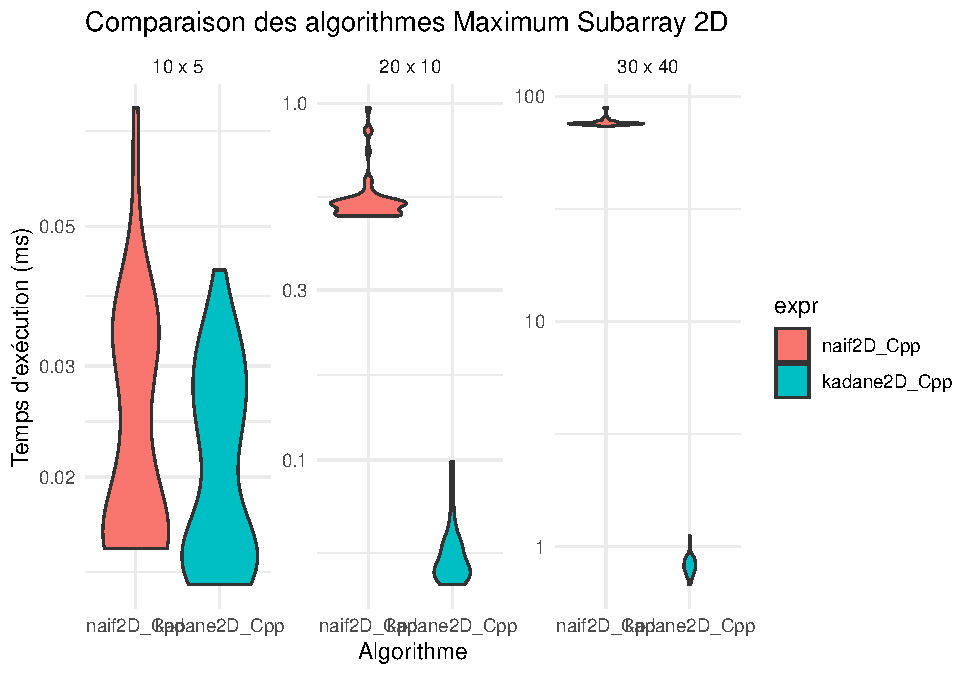
\includegraphics{MaxSubarray2D_files/figure-latex/benchmark-1.pdf}

\begin{verbatim}
## # A tibble: 6 x 8
##    size expr         min_time  q1_time median_time mean_time q3_time max_time
##   <dbl> <fct>           <dbl>    <dbl>       <dbl>     <dbl>   <dbl>    <dbl>
## 1    50 naif2D_Cpp     0.01    0.0105       0.0108    0.0118  0.0113   0.0331
## 2    50 kadane2D_Cpp   0.0085  0.00962      0.0104    0.0112  0.0114   0.0299
## 3   200 naif2D_Cpp     0.307   0.308        0.309     0.330   0.317    0.686 
## 4   200 kadane2D_Cpp   0.0288  0.0296       0.0320    0.0397  0.0372   0.153 
## 5  1200 naif2D_Cpp    45.0    46.4         47.5      47.5    48.6     51.1   
## 6  1200 kadane2D_Cpp   0.457   0.523        0.558     0.579   0.609    0.874
\end{verbatim}

\begin{center}\rule{0.5\linewidth}{0.5pt}\end{center}

\section{Evaluation de la
complexité}\label{evaluation-de-la-complexituxe9}

\subparagraph{Complexité expériementale
(naif)}\label{complexituxe9-expuxe9riementale-naif}

D'après la littérature, et comme expliquée précedemment, l'agorithme
naif a une complexité polynomiale en O((nm)\^{}3), içi nous essayons
d'exp

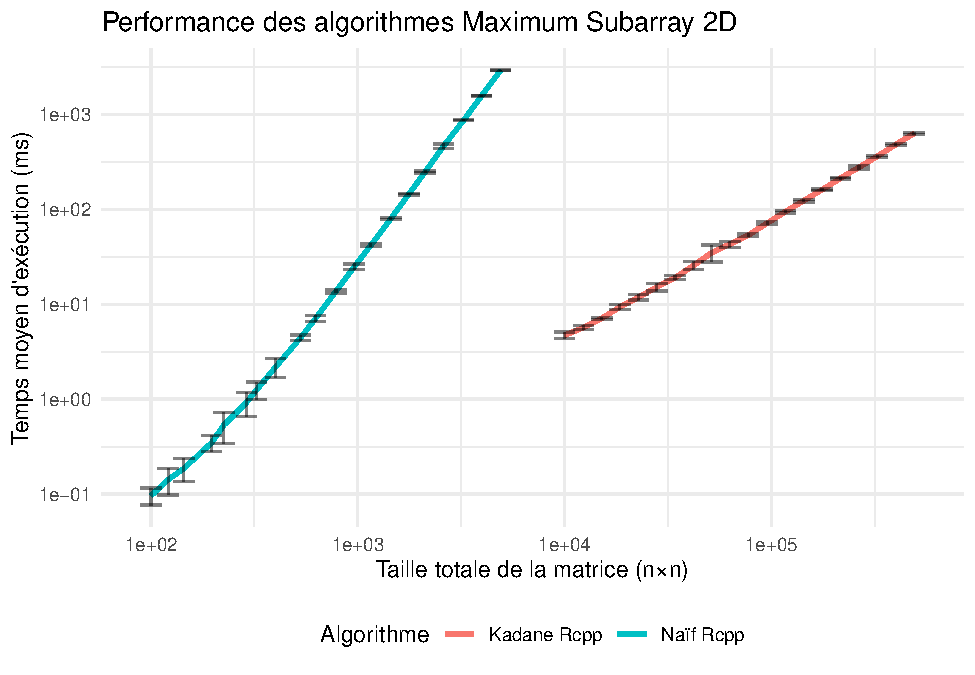
\includegraphics{MaxSubarray2D_files/figure-latex/simu complexite-1.pdf}

\begin{Shaded}
\begin{Highlighting}[]
\CommentTok{\# Affichage des résultats}
\FunctionTok{cat}\NormalTok{(}\StringTok{"Les résultats pour la solution naïve:"}\NormalTok{)}
\end{Highlighting}
\end{Shaded}

\begin{verbatim}
## Les résultats pour la solution naïve:
\end{verbatim}

\begin{Shaded}
\begin{Highlighting}[]
\NormalTok{res\_Naive\_2D}
\end{Highlighting}
\end{Shaded}

\begin{verbatim}
##     n  m mean_time     sd_time total_size
## 1  10 10     0.096  0.01955050        100
## 2  11 11     0.142  0.04417138        121
## 3  12 12     0.186  0.05168279        144
## 4  14 14     0.346  0.06801961        196
## 5  15 15     0.534  0.19265398        225
## 6  17 17     0.916  0.25872336        289
## 7  18 18     1.250  0.26115130        324
## 8  20 20     2.179  0.48098164        400
## 9  23 23     4.438  0.28549372        529
## 10 25 25     7.096  0.55349797        625
## 11 28 28    13.734  0.60415598        784
## 12 31 31    24.775  1.77162355        961
## 13 34 34    41.820  1.38223651       1156
## 14 38 38    79.585  2.10719535       1444
## 15 42 42   144.203  2.88942151       1764
## 16 46 46   247.426  5.94501509       2116
## 17 51 51   464.146 23.71130823       2601
## 18 57 57   866.553  9.57412723       3249
## 19 63 63  1564.906  7.49193967       3969
## 20 70 70  2907.218 25.18713199       4900
\end{verbatim}

\begin{Shaded}
\begin{Highlighting}[]
\FunctionTok{cat}\NormalTok{(}\StringTok{"Les résultats pour la solution optimale:"}\NormalTok{)}
\end{Highlighting}
\end{Shaded}

\begin{verbatim}
## Les résultats pour la solution optimale:
\end{verbatim}

\begin{Shaded}
\begin{Highlighting}[]
\NormalTok{res\_Kadane\_2D}
\end{Highlighting}
\end{Shaded}

\begin{verbatim}
##      n   m mean_time    sd_time total_size
## 1  100 100     4.699  0.3868520      10000
## 2  111 111     5.664  0.2813539      12321
## 3  123 123     7.092  0.2056318      15129
## 4  136 136     9.333  0.5034558      18496
## 5  151 151    11.866  0.8136229      22801
## 6  167 167    15.115  1.3503024      27889
## 7  185 185    19.008  0.9176516      34225
## 8  205 205    25.596  2.4731545      42025
## 9  227 227    34.937  7.0523236      51529
## 10 251 251    42.941  3.2107128      63001
## 11 278 278    53.335  1.7266297      77284
## 12 309 309    71.488  2.2730635      95481
## 13 342 342    94.241  2.9288392     116964
## 14 379 379   123.336  3.8497509     143641
## 15 419 419   160.155  3.7121011     175561
## 16 465 465   212.544  4.2603265     216225
## 17 515 515   276.896 11.4978067     265225
## 18 570 570   361.101  9.3000208     324900
## 19 632 632   480.394  9.7461060     399424
## 20 700 700   630.326 14.0494256     490000
\end{verbatim}

On vérifie la valeur du coefficient directeur pour les deux méthodes:

\begin{verbatim}
## 
## Call:
## lm(formula = log(res_Naive_2D$mean_time) ~ log(res_Naive_2D$n))
## 
## Residuals:
##      Min       1Q   Median       3Q      Max 
## -0.23073 -0.16716 -0.04825  0.12184  0.44446 
## 
## Coefficients:
##                     Estimate Std. Error t value Pr(>|t|)    
## (Intercept)         -15.2525     0.2465  -61.88   <2e-16 ***
## log(res_Naive_2D$n)   5.4133     0.0741   73.05   <2e-16 ***
## ---
## Signif. codes:  0 '***' 0.001 '**' 0.01 '*' 0.05 '.' 0.1 ' ' 1
## 
## Residual standard error: 0.1957 on 18 degrees of freedom
## Multiple R-squared:  0.9966, Adjusted R-squared:  0.9965 
## F-statistic:  5336 on 1 and 18 DF,  p-value: < 2.2e-16
\end{verbatim}

\begin{verbatim}
## Exposant estimé (naïf): 5.413324
\end{verbatim}

\begin{verbatim}
## 
## Call:
## lm(formula = log(res_Kadane_2D$mean_time) ~ log(res_Kadane_2D$n))
## 
## Residuals:
##       Min        1Q    Median        3Q       Max 
## -0.065266 -0.023608 -0.008487  0.021311  0.108724 
## 
## Coefficients:
##                       Estimate Std. Error t value Pr(>|t|)    
## (Intercept)          -10.28647    0.08876  -115.9   <2e-16 ***
## log(res_Kadane_2D$n)   2.54607    0.01582   160.9   <2e-16 ***
## ---
## Signif. codes:  0 '***' 0.001 '**' 0.01 '*' 0.05 '.' 0.1 ' ' 1
## 
## Residual standard error: 0.04175 on 18 degrees of freedom
## Multiple R-squared:  0.9993, Adjusted R-squared:  0.9993 
## F-statistic: 2.59e+04 on 1 and 18 DF,  p-value: < 2.2e-16
\end{verbatim}

\begin{verbatim}
## Exposant estimé (Kadane): 2.546071
\end{verbatim}

Les coefficients directeurs trouvés sont bien ceux que l'on attendait.
La valeur pour la méthode naïve 6 car \(O\left((nm)^3\right)\)~=
\(O\left((n^2)^3\right)\)~et 3 car \(O(n \cdot m^2)\) =
\(O(n \cdot n^2)\) pour l'algorithme de Kadane

\begin{center}\rule{0.5\linewidth}{0.5pt}\end{center}

\section{Cas particulier des données presques
triées}\label{cas-particulier-des-donnuxe9es-presques-triuxe9es}

On considère des données triées avec 5\% de valeurs échangées au hasard.

Sur un exemple cela donne :

\begin{Shaded}
\begin{Highlighting}[]
\CommentTok{\# Création d\textquotesingle{}une matrice triée}
\NormalTok{n }\OtherTok{\textless{}{-}} \DecValTok{10}  \CommentTok{\# nombre de lignes}
\NormalTok{m }\OtherTok{\textless{}{-}} \DecValTok{10}  \CommentTok{\# nombre de colonnes}
\NormalTok{v }\OtherTok{\textless{}{-}} \DecValTok{1}\SpecialCharTok{:}\NormalTok{(n }\SpecialCharTok{*}\NormalTok{ m)}
\NormalTok{n\_swap }\OtherTok{\textless{}{-}} \FunctionTok{floor}\NormalTok{(}\FloatTok{0.05} \SpecialCharTok{*} \FunctionTok{length}\NormalTok{(v))}
\NormalTok{swap\_indices }\OtherTok{\textless{}{-}} \FunctionTok{sample}\NormalTok{(}\FunctionTok{length}\NormalTok{(v), n\_swap)}
\NormalTok{v[swap\_indices] }\OtherTok{\textless{}{-}} \FunctionTok{sample}\NormalTok{(v[swap\_indices])}
\NormalTok{mat }\OtherTok{\textless{}{-}} \FunctionTok{matrix}\NormalTok{(v, }\AttributeTok{nrow =}\NormalTok{ n, }\AttributeTok{ncol =}\NormalTok{ m)}
\NormalTok{mat}
\end{Highlighting}
\end{Shaded}

\begin{verbatim}
##       [,1] [,2] [,3] [,4] [,5] [,6] [,7] [,8] [,9] [,10]
##  [1,]    1   11   21   31   41   51   61   71   81    91
##  [2,]    2   12   22   32   42   52   62   72   82    92
##  [3,]    3   13   23   33   18   53   63   73   83    93
##  [4,]    4   14   24   34   44   54   64   74   84    94
##  [5,]    5   15   25   35   45   55   65   75   85    95
##  [6,]    6   16   26   36   46   43   66   76   86    96
##  [7,]    7   17   27   37   47   57   67   77   87    97
##  [8,]    8   56   28   38   48   58   68   78   88    98
##  [9,]    9   19   29   39   49   59   69   79   89    99
## [10,]   10   20   30   40   50   60   70   80   90   100
\end{verbatim}

\begin{Shaded}
\begin{Highlighting}[]
\CommentTok{\# Fonctions de simulation}
\NormalTok{one.simu }\OtherTok{\textless{}{-}} \ControlFlowTok{function}\NormalTok{(n,m, func) \{}
\NormalTok{  mat }\OtherTok{\textless{}{-}} \FunctionTok{matrix}\NormalTok{(}\FunctionTok{sample}\NormalTok{(}\SpecialCharTok{{-}}\DecValTok{100}\SpecialCharTok{:}\DecValTok{100}\NormalTok{, n }\SpecialCharTok{*}\NormalTok{ m, }\AttributeTok{replace =} \ConstantTok{TRUE}\NormalTok{), }\AttributeTok{nrow =}\NormalTok{ n, }\AttributeTok{ncol =}\NormalTok{ m)}
  \ControlFlowTok{if}\NormalTok{ (func }\SpecialCharTok{==} \StringTok{"Naive2D\_cpp"}\NormalTok{) }\FunctionTok{return}\NormalTok{(}\FunctionTok{max\_subarray\_rectangle\_naive}\NormalTok{(mat))}
  \ControlFlowTok{if}\NormalTok{ (func }\SpecialCharTok{==} \StringTok{"Kadane2D\_cpp"}\NormalTok{) }\FunctionTok{return}\NormalTok{(}\FunctionTok{max\_subarray\_rectangle\_opt\_Rcpp}\NormalTok{(mat))}
\NormalTok{\}}

\NormalTok{one.simu2 }\OtherTok{\textless{}{-}} \ControlFlowTok{function}\NormalTok{(n,m, func) \{}
\NormalTok{  v }\OtherTok{\textless{}{-}} \DecValTok{1}\SpecialCharTok{:}\NormalTok{(n }\SpecialCharTok{*}\NormalTok{ m)}
\NormalTok{  n\_swap }\OtherTok{\textless{}{-}} \FunctionTok{floor}\NormalTok{(}\FloatTok{0.05} \SpecialCharTok{*} \FunctionTok{length}\NormalTok{(v))}
\NormalTok{  swap\_indices }\OtherTok{\textless{}{-}} \FunctionTok{sample}\NormalTok{(}\FunctionTok{length}\NormalTok{(v), n\_swap)}
\NormalTok{  v[swap\_indices] }\OtherTok{\textless{}{-}} \FunctionTok{sample}\NormalTok{(v[swap\_indices])}
\NormalTok{  mat }\OtherTok{\textless{}{-}} \FunctionTok{matrix}\NormalTok{(v, }\AttributeTok{nrow =}\NormalTok{ n, }\AttributeTok{ncol =}\NormalTok{ m)}
  \ControlFlowTok{if}\NormalTok{ (func }\SpecialCharTok{==} \StringTok{"Naive2D\_cpp"}\NormalTok{) }\FunctionTok{return}\NormalTok{(}\FunctionTok{max\_subarray\_rectangle\_naive}\NormalTok{(mat))}
  \ControlFlowTok{if}\NormalTok{ (func }\SpecialCharTok{==} \StringTok{"Kadane2D\_cpp"}\NormalTok{) }\FunctionTok{return}\NormalTok{(}\FunctionTok{max\_subarray\_rectangle\_opt\_Rcpp}\NormalTok{(mat))}
\NormalTok{\}}
\end{Highlighting}
\end{Shaded}

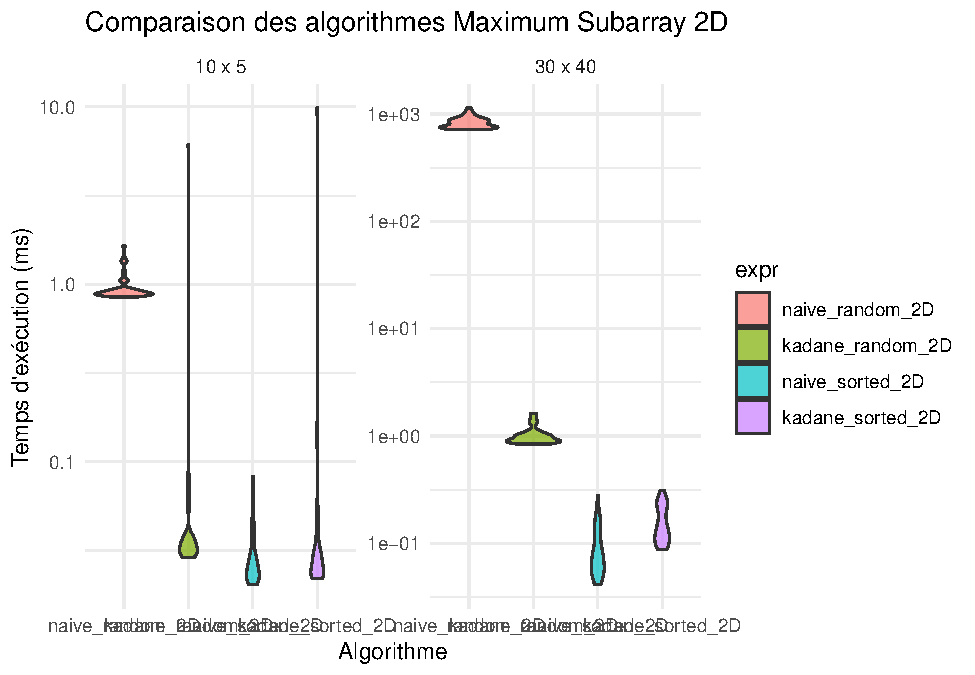
\includegraphics{MaxSubarray2D_files/figure-latex/benchmark2-1.pdf}

\begin{verbatim}
## # A tibble: 8 x 8
##    size expr             min_time q1_time median_time mean_time q3_time max_time
##   <dbl> <fct>               <dbl>   <dbl>       <dbl>     <dbl>   <dbl>    <dbl>
## 1    50 naive_random_2D    0.787  8.25e-1      0.868     1.07   1.34e+0   2.07  
## 2    50 kadane_random_2D   0.0263 2.75e-2      0.0308    0.177  4.91e-2   6.95  
## 3    50 naive_sorted_2D    0.0176 1.92e-2      0.0219    0.0289 3.02e-2   0.0723
## 4    50 kadane_sorted_2D   0.0185 2.02e-2      0.0233    0.256  3.10e-2  11.4   
## 5  1200 naive_random_2D  479.     5.12e+2    524.      558.     5.99e+2 711.    
## 6  1200 kadane_random_2D   0.539  5.66e-1      0.591     0.617  6.71e-1   0.908 
## 7  1200 naive_sorted_2D    0.0271 3.27e-2      0.0432    0.0566 6.15e-2   0.140 
## 8  1200 kadane_sorted_2D   0.0574 6.60e-2      0.0812    0.110  1.77e-1   0.196
\end{verbatim}

Pour \texttt{(n,m)\ =\ (10,5)}, le temps d'exécution est plus rapide que
pour \texttt{(n,m)\ =\ (30,40)}. Kadane est toujours plus rapide que
Naïf, avec un écart plus important à \texttt{(n,m)\ =\ (30,40)}. Lorsque
les tableaux sont triés, Naïf et Kadane sont beaucoup plus rapides, avec
un écart réduit entre les deux.

\section{Cas particulier avec matrice
symétrique}\label{cas-particulier-avec-matrice-symuxe9trique}

On considère une matrice symétrique

Sur un exemple cela donne :

\begin{Shaded}
\begin{Highlighting}[]
\CommentTok{\# Création d\textquotesingle{}une matrice triée}
\NormalTok{n }\OtherTok{\textless{}{-}} \DecValTok{10}  \CommentTok{\# nombre de lignes}
\NormalTok{m }\OtherTok{\textless{}{-}} \DecValTok{10}  \CommentTok{\# nombre de colonnes}

\NormalTok{v\_sym }\OtherTok{\textless{}{-}} \FunctionTok{sample}\NormalTok{(}\DecValTok{1}\SpecialCharTok{:}\DecValTok{100}\NormalTok{, n }\SpecialCharTok{*}\NormalTok{ m, }\AttributeTok{replace =} \ConstantTok{TRUE}\NormalTok{)}
\NormalTok{mat }\OtherTok{\textless{}{-}} \FunctionTok{matrix}\NormalTok{(v\_sym, }\AttributeTok{nrow =}\NormalTok{ n, }\AttributeTok{ncol =}\NormalTok{ m)}
\NormalTok{mat[}\FunctionTok{lower.tri}\NormalTok{(mat)] }\OtherTok{\textless{}{-}} \FunctionTok{t}\NormalTok{(mat)[}\FunctionTok{lower.tri}\NormalTok{(mat)]}
  
\NormalTok{mat}
\end{Highlighting}
\end{Shaded}

\begin{verbatim}
##       [,1] [,2] [,3] [,4] [,5] [,6] [,7] [,8] [,9] [,10]
##  [1,]   50   59   16   85   17   37   38   98   37    92
##  [2,]   59   52   11   76   85   92    8   24   89    14
##  [3,]   16   11   70   12   28   69   82   49   80    96
##  [4,]   85   76   12   86   32   16   81   41    6    56
##  [5,]   17   85   28   32   39   58   76   40   28    24
##  [6,]   37   92   69   16   58   93   44   16   24    90
##  [7,]   38    8   82   81   76   44   12   91   65    18
##  [8,]   98   24   49   41   40   16   91   15   65    38
##  [9,]   37   89   80    6   28   24   65   65   80    48
## [10,]   92   14   96   56   24   90   18   38   48    23
\end{verbatim}

\begin{Shaded}
\begin{Highlighting}[]
\CommentTok{\# Fonctions de simulation}
\NormalTok{one.simu }\OtherTok{\textless{}{-}} \ControlFlowTok{function}\NormalTok{(n,m, func) \{}
\NormalTok{  mat }\OtherTok{\textless{}{-}} \FunctionTok{matrix}\NormalTok{(}\FunctionTok{sample}\NormalTok{(}\SpecialCharTok{{-}}\DecValTok{100}\SpecialCharTok{:}\DecValTok{100}\NormalTok{, n }\SpecialCharTok{*}\NormalTok{ m, }\AttributeTok{replace =} \ConstantTok{TRUE}\NormalTok{), }\AttributeTok{nrow =}\NormalTok{ n, }\AttributeTok{ncol =}\NormalTok{ m)}
  \ControlFlowTok{if}\NormalTok{ (func }\SpecialCharTok{==} \StringTok{"Naive2D\_cpp"}\NormalTok{) }\FunctionTok{return}\NormalTok{(}\FunctionTok{max\_subarray\_rectangle\_naive}\NormalTok{(mat))}
  \ControlFlowTok{if}\NormalTok{ (func }\SpecialCharTok{==} \StringTok{"Kadane2D\_cpp"}\NormalTok{) }\FunctionTok{return}\NormalTok{(}\FunctionTok{max\_subarray\_rectangle\_opt\_Rcpp}\NormalTok{(mat))}
\NormalTok{\}}

\NormalTok{one.simu2 }\OtherTok{\textless{}{-}} \ControlFlowTok{function}\NormalTok{(n,m, func) \{}
\NormalTok{  v\_sym }\OtherTok{\textless{}{-}} \FunctionTok{sample}\NormalTok{(}\DecValTok{1}\SpecialCharTok{:}\DecValTok{100}\NormalTok{, n }\SpecialCharTok{*}\NormalTok{ m, }\AttributeTok{replace =} \ConstantTok{TRUE}\NormalTok{)}
\NormalTok{  mat }\OtherTok{\textless{}{-}} \FunctionTok{matrix}\NormalTok{(v\_sym, }\AttributeTok{nrow =}\NormalTok{ n, }\AttributeTok{ncol =}\NormalTok{ m)}
\NormalTok{  mat[}\FunctionTok{lower.tri}\NormalTok{(mat)] }\OtherTok{\textless{}{-}} \FunctionTok{t}\NormalTok{(mat)[}\FunctionTok{lower.tri}\NormalTok{(mat)]}
  \ControlFlowTok{if}\NormalTok{ (func }\SpecialCharTok{==} \StringTok{"Naive2D\_cpp"}\NormalTok{) }\FunctionTok{return}\NormalTok{(}\FunctionTok{max\_subarray\_rectangle\_naive}\NormalTok{(mat))}
  \ControlFlowTok{if}\NormalTok{ (func }\SpecialCharTok{==} \StringTok{"Kadane2D\_cpp"}\NormalTok{) }\FunctionTok{return}\NormalTok{(}\FunctionTok{max\_subarray\_rectangle\_opt\_Rcpp}\NormalTok{(mat))}
\NormalTok{\}}
\end{Highlighting}
\end{Shaded}

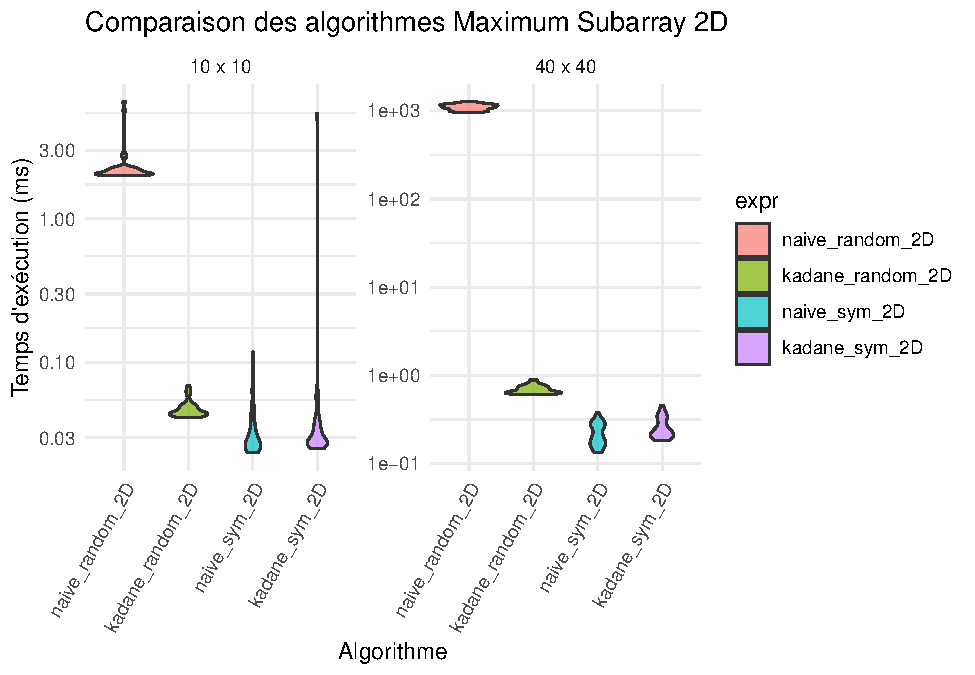
\includegraphics{MaxSubarray2D_files/figure-latex/benchmark3-1.pdf}

\begin{verbatim}
## # A tibble: 8 x 8
##    size expr             min_time q1_time median_time mean_time q3_time max_time
##   <dbl> <fct>               <dbl>   <dbl>       <dbl>     <dbl>   <dbl>    <dbl>
## 1   100 naive_random_2D    1.99   2.04e+0      2.10      2.31   2.23e+0  6.52e+0
## 2   100 kadane_random_2D   0.0414 4.34e-2      0.045     0.0476 4.98e-2  6.92e-2
## 3   100 naive_sym_2D       0.0236 2.55e-2      0.0281    0.0353 3.70e-2  1.18e-1
## 4   100 kadane_sym_2D      0.0254 2.72e-2      0.0287    0.140  3.59e-2  5.41e+0
## 5  1600 naive_random_2D  962.     1.02e+3   1094.     1101.     1.17e+3  1.27e+3
## 6  1600 kadane_random_2D   0.612  6.32e-1      0.658     0.691  7.35e-1  8.88e-1
## 7  1600 naive_sym_2D       0.132  1.68e-1      0.205     0.220  2.81e-1  3.81e-1
## 8  1600 kadane_sym_2D      0.182  2.04e-1      0.226     0.258  3.14e-1  4.53e-1
\end{verbatim}

Pour \texttt{(n,m)\ =\ (10,10)}, le temps d'exécution est plus rapide
que pour \texttt{(n,m)\ =\ (40,40)}. Kadane est toujours plus rapide que
Naïf, avec un écart plus important à \texttt{(n,m)\ =\ (40,40)}. Lorsque
les tableaux sont symétriques, Naïf et Kadane sont beaucoup plus
rapides, avec un écart réduit entre les deux.

\end{document}
